\begin{frame}
	\titlepage
	% Achtergrond, stagebedrijf etc.
\end{frame}

\begin{frame}{Huidig scorebord}
	\begin{itemize}
		\item Arbeidsitensief.
		\item Ontoereikende lichtopbrengst.
		\item Afhankelijk van externe computer.
		\item Storingsgevoelige draadloze bediening.
	\end{itemize}
\end{frame}

\begin{frame}{Concept Scorebord 2}
	\begin{itemize}
		\item Geen mechanische onderdelen.
		\item Plaatsen van de leds is minder arbeidsintensief.
		\item Niet meer afhankelijk van een externe computer.
		\item Draadloos te bedienen.
	\end{itemize}
\end{frame}

\begin{frame}{Doelstelling}
	%Demonstratie van ledpanelen.
	\begin{itemize}
		\item Realiseer een animatie en een score op een matrix van 2x4 ledpanelen.
	\end{itemize}
\end{frame}

\begin{frame}{Communicatie tussen de ledpanelen en de ECU}
	Hardware:
	\begin{itemize}
		\item CAN-bus.
	\end{itemize}
	
	Software:
	\begin{itemize}
		\item Ledscherm communicatieprotocol.
		\item Busstreamer
		\item CAN-wrapper
	\end{itemize}
\end{frame}

\begin{frame}
	\begin{figure}[h]
		\centering
		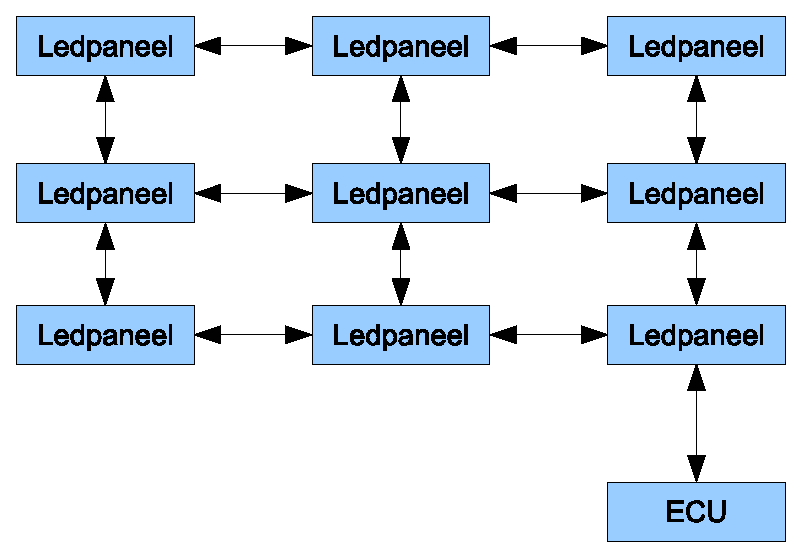
\includegraphics[width=10cm]{figuren/bussysteem}
		\caption{Netwerk van ledpanelen en de ECU.}
	\end{figure}
\end{frame}

\begin{frame}{Software op de ECU}
	\begin{itemize}
		\item Videoframeprogramma's.
			\begin{itemize}
				\item clientsoftware
					\begin{itemize}
						\item gif/png streamer.
						\item tekencanvas.
						\item pong.
						\item videostreamer.
					\end{itemize}
			\end{itemize}
		\item Ledschermdriver (software modules).
			\begin{itemize}
				\item ledschermserver.
				\item layers.
				\item busstreamer.
			\end{itemize}
	\end{itemize}
\end{frame}

\begin{frame}{Software van de ledpanelen.}
	Software modules:
	\begin{itemize}
		\item Ledscherm communicatieprotocol.
		\item Busstreamer.
		\item CAN-wrapper.
		\item Positioneringssysteem.
	\end{itemize}
\end{frame}

\begin{frame}{Positioneringssysteem}
	Het positioneringssysteemalgoritme bestaat uit de volgende toestanden:
	\begin{itemize}
		\item STATE\textunderscore DAISY\textunderscore UP
		\item STATE\textunderscore FEEL
		\item STATE\textunderscore DAISY\textunderscore DOWN
		\item STATE\textunderscore NODE\textunderscore KNOWN
		\item STATE\textunderscore NODE\textunderscore UNKNOWN
		\item STATE\textunderscore NODE\textunderscore OPERATIONAL
	\end{itemize}
\end{frame}

\begin{frame}{Positioneringssysteem}
	% animatie.
	\begin{figure}[h]
		\centering
		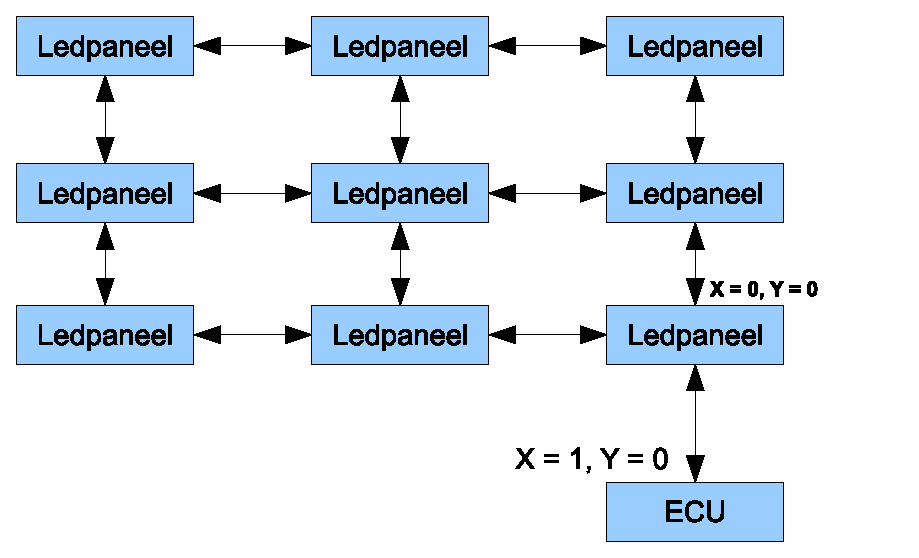
\includegraphics[width=12cm]{animatie/0}
		\caption{Netwerk van ledpanelen en de ECU.}
	\end{figure}
\end{frame}

\begin{frame}{Positioneringssysteem}
	% animatie.
	\begin{figure}[h]
		\centering
		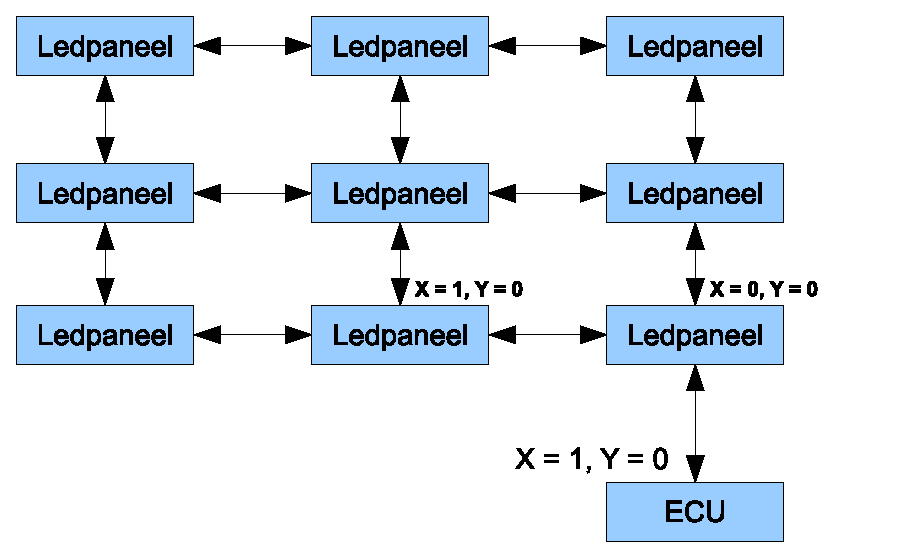
\includegraphics[width=12cm]{animatie/1}
		\caption{Netwerk van ledpanelen en de ECU.}
	\end{figure}
\end{frame}

\begin{frame}{Positioneringssysteem}
	% animatie.
	\begin{figure}[h]
		\centering
		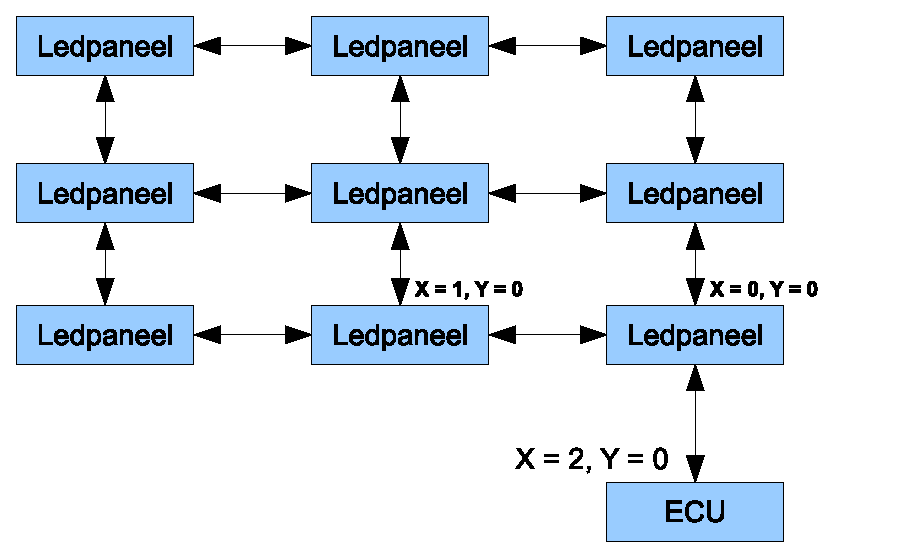
\includegraphics[width=12cm]{animatie/2}
		\caption{Netwerk van ledpanelen en de ECU.}
	\end{figure}
\end{frame}

\begin{frame}{Positioneringssysteem}
	% animatie.
	\begin{figure}[h]
		\centering
		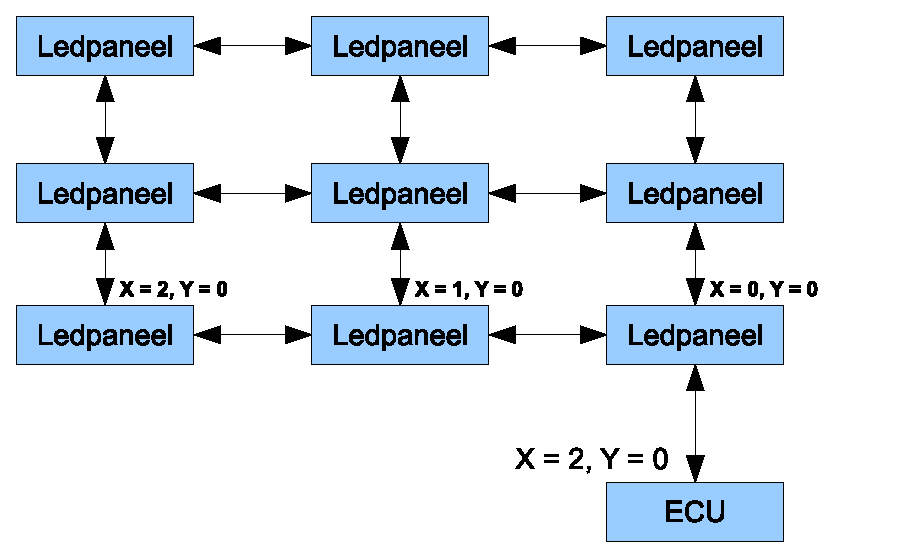
\includegraphics[width=12cm]{animatie/3}
		\caption{Netwerk van ledpanelen en de ECU.}
	\end{figure}
\end{frame}

\begin{frame}{Positioneringssysteem}
	% animatie.
	\begin{figure}[h]
		\centering
		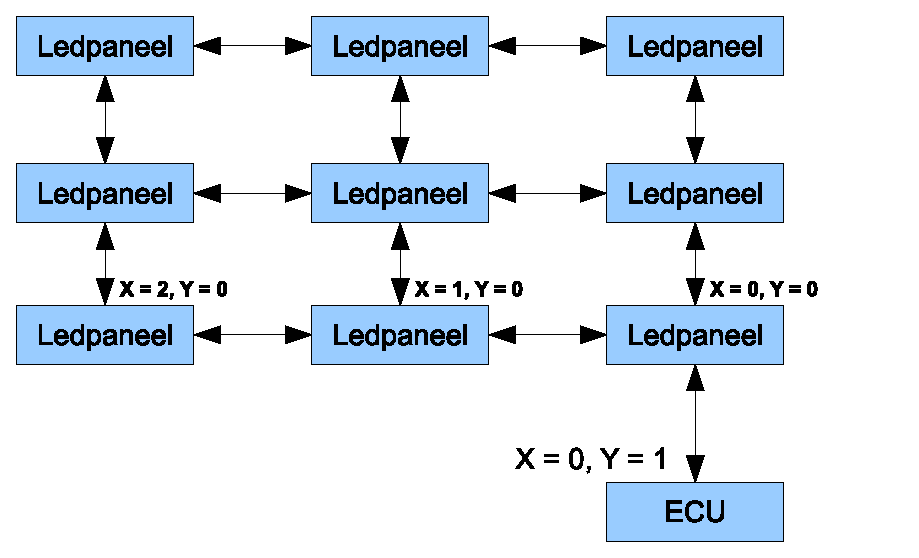
\includegraphics[width=12cm]{animatie/4}
		\caption{Netwerk van ledpanelen en de ECU.}
	\end{figure}
\end{frame}

\begin{frame}{Positioneringssysteem}
	% animatie.
	\begin{figure}[h]
		\centering
		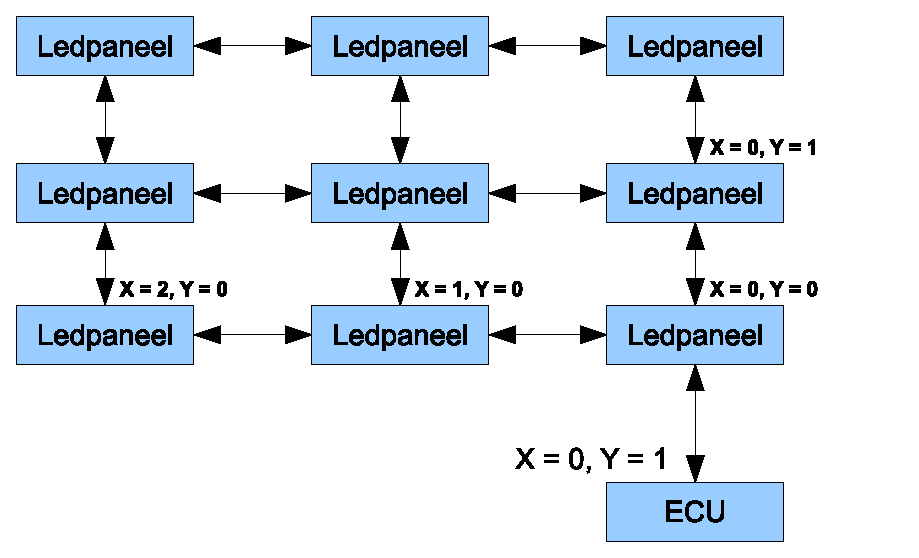
\includegraphics[width=12cm]{animatie/5}
		\caption{Netwerk van ledpanelen en de ECU.}
	\end{figure}
\end{frame}

\begin{frame}{Positioneringssysteem}
	% animatie.
	\begin{figure}[h]
		\centering
		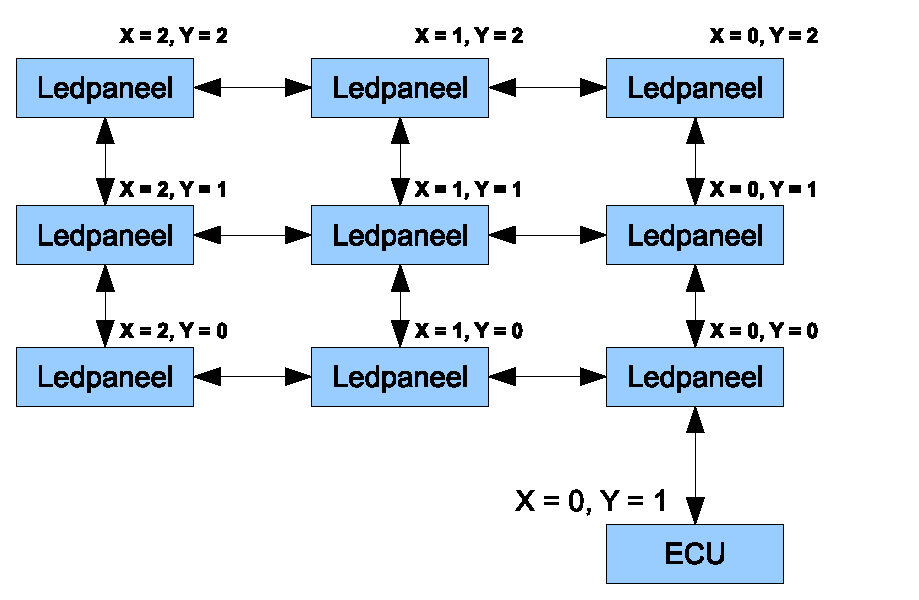
\includegraphics[width=12cm]{animatie/6}
		\caption{Netwerk van ledpanelen en de ECU.}
	\end{figure}
\end{frame}

\begin{frame}{Positioneringssysteem}
	% animatie.
	\begin{figure}[h]
		\centering
		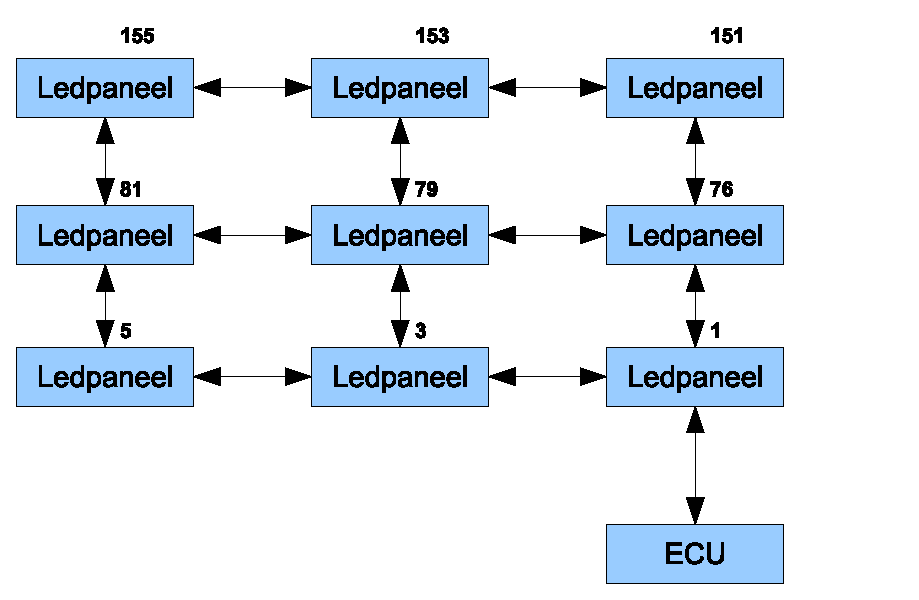
\includegraphics[width=12cm]{animatie/7}
		\caption{Netwerk van ledpanelen en de ECU.}
	\end{figure}
\end{frame}

\begin{frame}{Metingen}
	\begin{table}[h]
		\begin{tabular}{lllll}
		Aantal ledpanelen	& FPS 		& tijdsduur 	& compressieratio \\
		\hline
		\end{tabular}
		\caption{Compressieratio gebaseerd op gemeten waarde.}
	\end{table}
\end{frame}

\begin{frame}{Conclusie}
	Onderzoek
	\begin{itemize}
		\item Vergelijkbare systemen.
		\item Positioneringssysteem.
		\item Dataoverdracht.
		\item Bussystemen.
	\end{itemize}
\end{frame}

\begin{frame}
	%Vervolg.
	Ontwerp en implementaties:
	\begin{itemize}
		\item Videoframesoftware (tonen van gif/png animaties en afbeeldignen, ledscherm als tekencanvas)
		\item Ledschermdriver:
			\begin{itemize}
				\item Ledschermserver
				\item Imageprocessing (Layers, cropper)
				\item Linked-list.
				\item Busstreamer.
			\end{itemize}
		\item Ledpaneelsoftware:
			\begin{itemize}
				\item Ledscherm communicatieprotocol;
				\item Positioneringssysteem.
				\item Buswrapper.
			\end{itemize}
		\item Gemeenschappelijke softwaremodules:
			\begin{itemize}
				\item Typeconversion.
			\end{itemize}
	\end{itemize}
	Metingen.
\end{frame}

\begin{frame}{Aanbevelingen}
	\begin{itemize}
		\item Optie 1:
		\item Optie 2:
	\end{itemize}	
\end{frame}